\documentclass[tikz]{standalone}
\usepackage{tikz}

% Global settings
\tikzset{
    every picture/.style={
        line width=0.2mm,
        dashed line/.style={dashed, opacity=0.6}
    },
    % Style for centered labels
    area label/.style={
        font=\sffamily,
        align=center
    }
}

% Define semantic color names (keeping exact same RGB values)
\definecolor{senderArea}{RGB}{204,255,204}  % Light green
\definecolor{postageArea}{RGB}{204,229,255} % Light blue
\definecolor{marginArea}{RGB}{255,204,204}  % Light red
\definecolor{codeArea}{RGB}{255,229,204}    % Light orange
\definecolor{readingArea}{RGB}{204,255,255} % Light cyan

\begin{document}
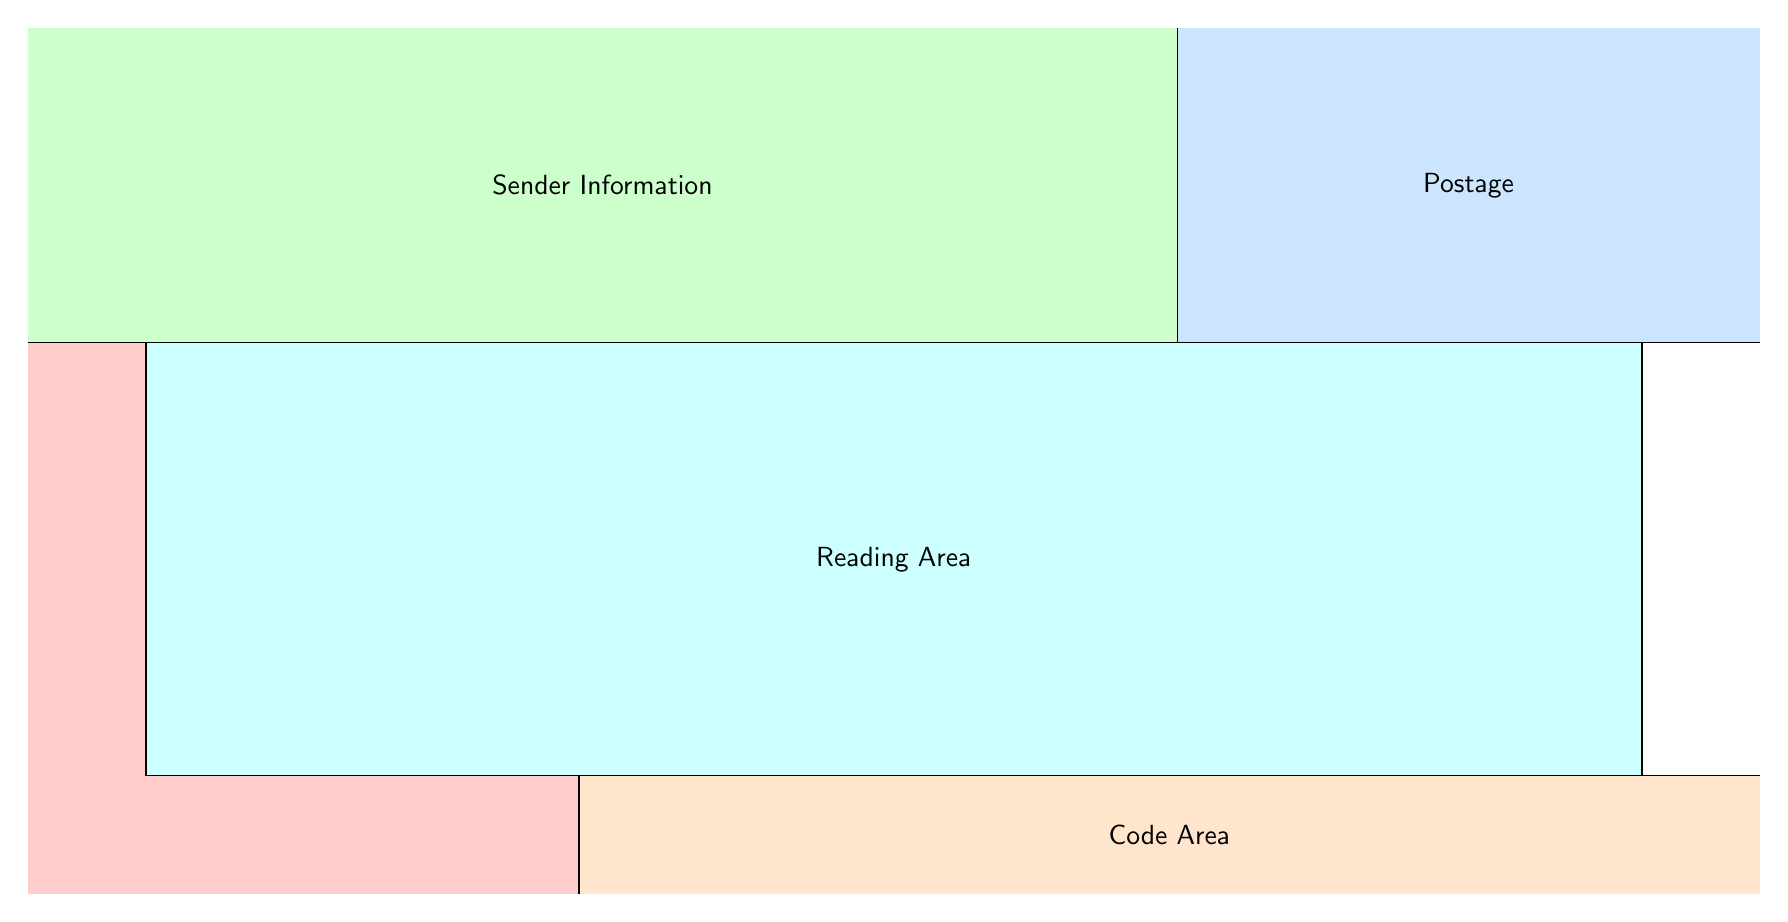
\begin{tikzpicture}[x=1mm,y=1mm]

% Set the canvas size
\path[use as bounding box] (0,0) rectangle (220,110);

% Draw all filled areas with centered labels
\fill[senderArea] (0,70) rectangle ++(146,40);
\node[area label] at (73,90) {Sender Information};

\fill[postageArea] (146,70) rectangle ++(74,40);
\node[area label] at (183,90) {Postage};

\fill[marginArea] (0,0) rectangle ++(15,70);
\fill[marginArea] (15,0) rectangle ++(55,15);

\fill[codeArea] (70,0) rectangle ++(150,15);
\node[area label] at (145,7.5) {Code Area};

\fill[readingArea] (15,15) rectangle ++(190,55);
\node[area label] at (110,42.5) {Reading Area};

% Draw all dashed lines
\draw(0,70) -- (146,70);
\draw(146,70) -- (146,110);
\draw(146,70) -- (220,70);
\draw(15,15) -- (15,70);
\draw(70,0) -- (70,15);
\draw(15,15) -- (70,15);
\draw(70,15) -- (220,15);
\draw(205,15) -- (205,70);

\end{tikzpicture}
\end{document}